%************************************************
%\chapter{An alternative structure to a blockchain: Confirmations without blocks}
%************************************************

\chapter{Introduction}

Bitcoin (BTC) is the first digital currency, also known as digital money, internet money and cryptocurrency. It is the first currency based on cryptography techniques, distributed and decentralized, and with no central bank. Bitcoin is distributed since its ledger is public and is stored in thousands of computers. It is decentralized because there is no authority (or government) who decides its future --- any decision must be accepted by its community. The security of Bitcoin relies on digital signature technology, so the owner of some BTC tokens is, in fact, the owner of a pair of private and public keys. One may either use the private key to transfer some tokens to another, or use the public key to a proof-of-ownership. If one looses their private key, unfortunately, access to their coins will be lost forever.

Since 2009, Bitcoin has been growing and becoming widely used all around the world. It started as an experiment based in a seminal work from \citet{nakamoto2008bitcoin} and expanded to the most important and successful cryptocurrency with a \$36 billion market capitalization \citep{coinmarketcapbtc}. There are hundreds of companies investing in different uses of the technology, from exchanges to debit cards, and billions of dollars being invested in the new markets created by Bitcoin.

The main problem when one is trying to create a digital money is how to prevent double spending. As the money is digital, what would prevent counterfeiting? That is, what would prevent users from sending copies of the same money to two (or more) people? That is exactly the problem solved by Bitcoin and its underlying blockchain technology. The current solution behind fiat money is having a single issuer, a central bank, and trusting the financial institutions.

Despite Bitcoin's huge success, there are still many challenges to be overcome. The network must scale to support hundreds of transactions per second, but today its capacity is close to 8 transactions per second. Another important challenge is to reduce the size of the ledger (or blockchain), which today is around 125GB and is growing at a rate of 4.5GB per month \citep{blockchaininfosize}.

Bitcoin has the most decentralized network between the cryptocurrencies, even so there are few miners and mining pools which together control over 50\% of the network’s computing (hash)power. Thus, they have an oversized influence when it comes to changes in the Bitcoin protocol's behaviour, and it is seen as a problem to be solved.

According to \citet{barber2012bitter}, despite the 30-year literature on e-cash, most of the proposed schemes requires a central authority which controls the currency issuance and prevents double spending. The no central point of trust and predictable money supply together with a clever solution to the double spending problem is what separates Bitcoin from the e-cash literature.

The number of ideas and publications focusing in improving Bitcoin's design is increasing every day. Many of these proposals are organized into BIPs (Bitcoin Improvement Proposals) which are discussed and implemented by the community; while others come in the form of whitepapers and alternative software forks (which would include the need of a protocol upgrade). Other scaling proposals are published in blogs and forums, describing new cryptocurrencies. Bitcoin's community hardly ever publishes their ideas in academic journals.

% Spam problem.

%The DAG model \citep{dagdiscussion2014, tangle2016, dagcoin2015, sompolinsky2013, lewenberg2015, vorick2015} has a different design which has neither mining nor confirmation blocks and transaction fees. Each transaction has its own proof-of-work, and is used to confirm other transactions in a directed acyclic graph. Although this design has been used by a few cryptocurrencies, none of them has enough users and would strengthen that the problems have been solved.

The DAG model \citep{dagdiscussion2014, tangle2016, dagcoin2015, sompolinsky2013, lewenberg2015, vorick2015} has different design which has neither mining nor confirmation blocks and transaction fees. Each transaction has its own proof-of-work, and is used to confirm other transactions in a directed acyclic graph. The present work intends to analyze whether the DAG model may be a viable solution to both Bitcoin's scaling problem and Bitcoin's oversized influence of a few miners and mining pools.

\chapter{Bitcoin \& Blockchain}

In \citeauthor{nakamoto2008bitcoin}'s (2009) seminal paper, there is no distinction between bitcoin and blockchain. They are just one thing which solves an important theoretical problem: how to create a distributed and decentralized digital form of hard money in the internet, in which all users can agree as to whom is entitled to which funds.

But, in practice, it is interesting to separate these concepts. Bitcoin uses the blockchain technology to create a distributed ledger, while the blockchain is a technology which allows information to be stored in an immutable and distributed way.

The blockchain technology works through the creation of new blocks. Each new block confirms that all the previous blocks are valid and have not been tampered with. The mechanism that assures the immutability is proof-of-work, which makes it computationally infeasible to tamper with previous transaction records without having to recalculate all the previous proof-of-works faster than all of the remaining machines of the network.

The proof-of-work is a mathematical problem with the following characteristics: (i) it is hard to find a solution; (ii) this difficulty level may be adjusted; and (iii) it is fast to check whether the proposed solution is correct.

Bitcoin's blockchain uses the mathematical problem of finding a random number which, after being applied to the hash function SHA-256 twice, results in a number smaller than a given number. As SHA-256 is a pseudo-random function, its output is uniformly distributed between 0 and $2^{256}-1$ \citep{gilbert2003security}. Thus, if the given number is $2^{255}$, one has probability 50\% of finding a solution (just the most significant bit of the hash needs to be zero). But if the given number is $2^{240}$, one has probability 0.0015\% of finding a solution (as the ~16 most significant bits of the hash must equal zero). Hence, finding a solution is a hard problem which difficulty depends on the given number. The lesser the given number, the higher the difficulty. On the other side, checking whether a solution is correct is fast, one just has to apply the SHA-256 twice and compare.

By design, Bitcoin's blockchain proof-of-work difficulty is dynamically adjusted every 2016 blocks to keep an average pace of 10 minutes between block creation. Thus, the goal is to adjust the difficulty every 14 days. If it takes less than 14 days to find 2016 blocks, that means the network's hash power has increased, thus the difficulty is increased. If it takes more than 14 days to find 2016 blocks, it means the network's hash power has decreased, thus the difficulty is decreased.

When miners are finding a solution to a new block, they are mining or working in the new block. A block is found when a solution to the proof-of-work is found. Two miners may find blocks in a small interval of time. In this case, both will propagate their blocks and the network will randomly choose one of them as the next block. This phenomenon is called a fork. Thus, when the next block is found, one of those blocks will be confirmed and the other will be ignored and referred to as an orphan block. The network agrees that work should be done in the block at the longest chain in the blockchain. When a new block is found, it indirectly confirms all the previous blocks in the chain and their transactions.

Newly propagated blocks are validated by the Bitcoin's network. If the solution of the proof-of-work is incorrect or if any transaction included in the block has any issue, then the block is discarded. In order to work properly, the whole network must agree in what is allowed and what is not. Should one think that something should be allowed and accept it in their blocks, the remaining of the network will discard their newly propagated blocks. That is why Bitcoin's network is distributed and decentralized. Everything depends on the agreement of the network, or, precisely, the agreement of the owners of at least 50\% of the hash power. Even if the remaining 49\% disagrees, the 50\% or more who agree will generate, on average, more blocks than the remaining of the network and their rules will prevail on the longest chain. If a disagreement between miners' rules happens, that is referred as either a hard-fork or a soft-fork (in general, a hard-fork relaxes the constraints, while the latter hardens them).

For instance, no group with more than 50\% of the network's hash power agreed into increasing the maximum block size to increase the number of transactions confirmed by a block, and thus increasing the network's capacity. Thus, the capacity remains the same and the community has been discussing the issue in search of a consensus.

Bitcoin uses the blockchain technology to create a distributed ledger. It allows every new block to generate new bitcoins and also to collect the fees from the confirmed transactions within the block. Bitcoin's transactions have two main parts: (i) inputs, and (ii) outputs. Each transaction sends bitcoins from one or more input addresses to one or more output addresses. In order to prove that one is the owner of the input bitcoins, one must digitally sign the transaction proving such ownership.

Bitcoins (BTCs) owned by someone are, in fact, unspent outputs in one or more transactions. For instance, one may have 6 BTCs spread between three transactions' unspent output: the first with 1 BTC, the second with 2 BTCs, and the third with 3 BTCs.

In a transaction, the inputs are pointers to other transactions' outputs (which they are spending). A transaction output may only be spent once and thus may not be partially spent. For instance, when one has 3 BTCs in one transaction output and would like to send 1 BTC to a friend, they have to create a transaction with one input spending the 3 BTCs and two outputs, one for the friend with 1 BTC and one's change with 2 BTCs. This enables $O(1)$ unspent transaction lookup.

Each transaction's output has a script that is executed by the miners to check whether one has or has not permission to spend that output. In other words, whether one has the ownership of that output. In order to execute these scripts, the miners also need some data. This data is given by the transaction which is spending the output.

The output's scripts usually checks whether the public key is valid and whether the digital signature was signed by the private key associated to that public key. Although there are only 3 commonly used scripts, one may create a custom script using the Bitcoin's script language \footnote{Your courageous author once tried to make a transaction with custom script to try to double spend a deposit to an exchange, only to learn through this intrepid adventure that Bitcoin allows only 3 script patterns and the others are treated as invalid.}.

The input contains the data which prove that the sender is the owner of the referred outputs, i.e., the input which must be accepted by the output scripts being spent. Usually, each input has the public key of the sender and a digital signature.

Those users accustomed to block explorers may have been misled by the transaction information that these websites provide.  For example, suppose a miner receives a transaction with ``one input from address A1''.  This ``one input'' actually consists of a pointer to a previous unspent output (i.e., there is no ``input'' address, as is displayed, but only a pointer). This pointer reference allows lookup to be executed in $O(1)$ time. 

After lookup, the miner knows how many BTC tokens are available at that unspent output.  But, in order to certify ownership of that output, the miner receives instructions in the form of a script with the rules that lead to the desired unspent output address (and this one is displayed as the input address by those websites). Because this process requires a digital signature, only the holder of the corresponding private key is able to sign such a transaction.

\chapter{DAG model}

DAG model proposes a whole different approach to confirmations. It proposes that there is no need for a block to confirm transactions, as transactions can confirm themselves. Here, each transaction has its own proof-of-work, named weight, and they must confirm two other, previous, transactions. Hence, each transaction has an accumulated weight, which is the accumulated proof-of-work that has confirmed it so far. In this sense, instead of a chain of blocks, the transactions and their confirmations form a directed and acyclic graph, as in Fig. \ref{fig-tangle-example}.

Like the Blockchain, the DAG model is another technology to store immutable data and may be the underlying technology to different applications, such as cryptocurrencies, digital contracts (Ethereum-like), digital notaries, and so forth. The main question which this work proposes to answer is: Is it reliable to use DAG model? In which conditions?

The transactions may be either confirmed or unconfirmed. The confirmed transactions have been already confirmed by at least one more transaction. It does not mean they are already irreversible and protected against a double spend attack --- it just means at least one transaction has done some work to confirm it. The unconfirmed transactions are called tips and they are eager to be confirmed. Usually a new transaction selects two tips to confirm, but this rule may not be followed.

Transactions may have any format, including Bitcoin-like transactions---with inputs, outputs, and scripts. But it also may be completely different, just like in the cryptocurrency Iota \citep{tangle2016}. This work will not discuss details of the transactions' format, because we understand that it does not affect exactly the network scalability and security.

\begin{figure}[ht]
\centering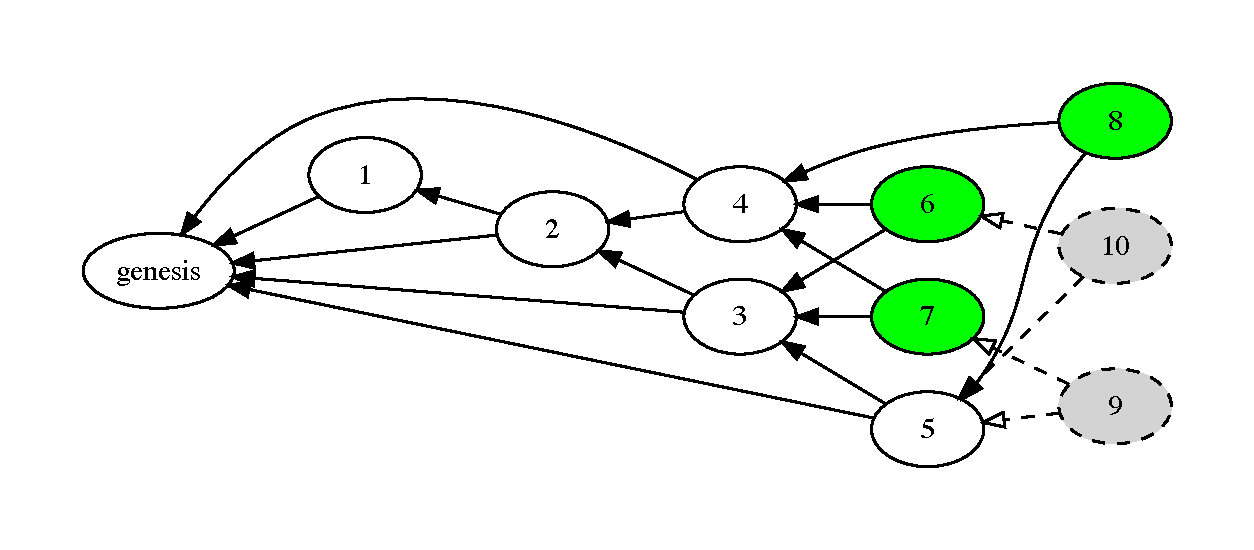
\includegraphics[width=\textwidth]{./images/fig-tangle-example.pdf}
\caption{White nodes represent transactions that have been confirmed at least once. Green circles represent unconfirmed transactions (tips). Gray and dashed nodes are the transactions currently solving the proof-of-work in order to be propagated.\label{fig-tangle-example}}
\end{figure}

The accumulated weight of a transaction A is the sum of all weights of the transactions which confirm A, including A itself, i.e., $w_A + \sum_{A \leadsto P} w_P$. For example, in Fig. \ref{fig-tangle-example}, the accumulated weight of transaction 3 is the sum of the weights of the transactions 5, 6, 7, and 8. The accumulated weight may be interpreted as how hard it is to rollback a transaction. It is analogous to the number of confirmations of a block in Bitcoin.

The score of a transaction A is the sum of all weights of the transactions which are being confirmed by A, including A itself, i.e., $w_A + \sum_{P \leadsto A} w_P$. For example, in Fig. \ref{fig-tangle-example}, the score of transaction 3 is the sum of the weights of the transactions 1 and 2. It is a measure of how much proof-of-work has been done before confirming this transaction. It may indicate whether the confirmed transactions have received enough attention (and hashpower) or whether it may have received tangential attention.

The height of a transaction A is the length of the longest path from transaction A to the genesis transaction. For example, in Fig. \ref{fig-tangle-example}, the height of transaction 5 is four ($5 \rightarrow 3 \rightarrow 2 \rightarrow 1 \rightarrow$ genesis). It may be interpreted as the “`age'' of the transaction. The lower the height, the older the transaction.

The depth of a transaction A is the length of the longest path in the inverted graph from transaction A to any unconfirmed transaction (tip). For example, in Fig. \ref{fig-tangle-example}, the depth of transaction 2 is three ($2 \rightarrow 3 \rightarrow 5 \rightarrow 8$). It is the opposite of the height. It may be interpreted as the youth of the transaction. The lower the depth, the younger the transaction. When a new transaction is confirming two transactions with high depth, it is referred as lazy transaction.

An important factor of DAG model is how the new transactions choose which transactions they will confirm. There are several possible approaches, such as randomly selecting two of the unconfirmed transactions (tips). In Fig \ref{fig-tangle-example}, the reader may have noticed that transaction 8 will confirm transaction 4, which has already been confirmed by transaction 7. It may be on purpose, or maybe transaction 4 was unconfirmed when it was chosen, but it got confirmed during the calculation of the proof-of-work or the network propagation of the transaction. The selection algorithm seems to be important to protect the network against double spend attacks.

The higher the volume of new transactions, the more unconfirmed transactions will appear. In Fig. \ref{fig-tangle-swarm}, the reader can notice that the number of new transactions was increased for a while, and then decreased back to the original value. The DAG has behaved well when exposed to a high load scenario, since it reduced the number of tips to only three. It is like a moving swarm which gets wider when the number of new transactions increases and gets thinner when the number of new transactions decreases.

\begin{figure}[ht]
\centering
\includegraphics[width=\textwidth]{./images/fig-tangle-swarm.pdf}
\caption{Suddenly the number of transactions per second increases and the width of the swarm grows. After a while, the number of transactions per second decreases and the width of the swarm shrinks.\label{fig-tangle-swarm}}
\end{figure}

Conflicting transactions may happen when two or more transactions try to spend the ``same money'' --- or, in the Bitcoin's transaction format, try to spend the same output. In this case, the network must choose which of the transactions will be accepted and the other one will be invalidated, even when both have already been confirmed. In fact, when one transaction is invalidated, the whole sub-DAG which confirms it is also invalidated. In this case, it may happen to reverse some transactions.

Intuitively, when there is a conflict, the network should accept the transaction which has greater accumulated weight, invalidating the others (see Fig. \ref{fig-tangle-conflict}). But it may be not enough to prevent a nuclear submarine attack.

\begin{figure}[ht]
\centering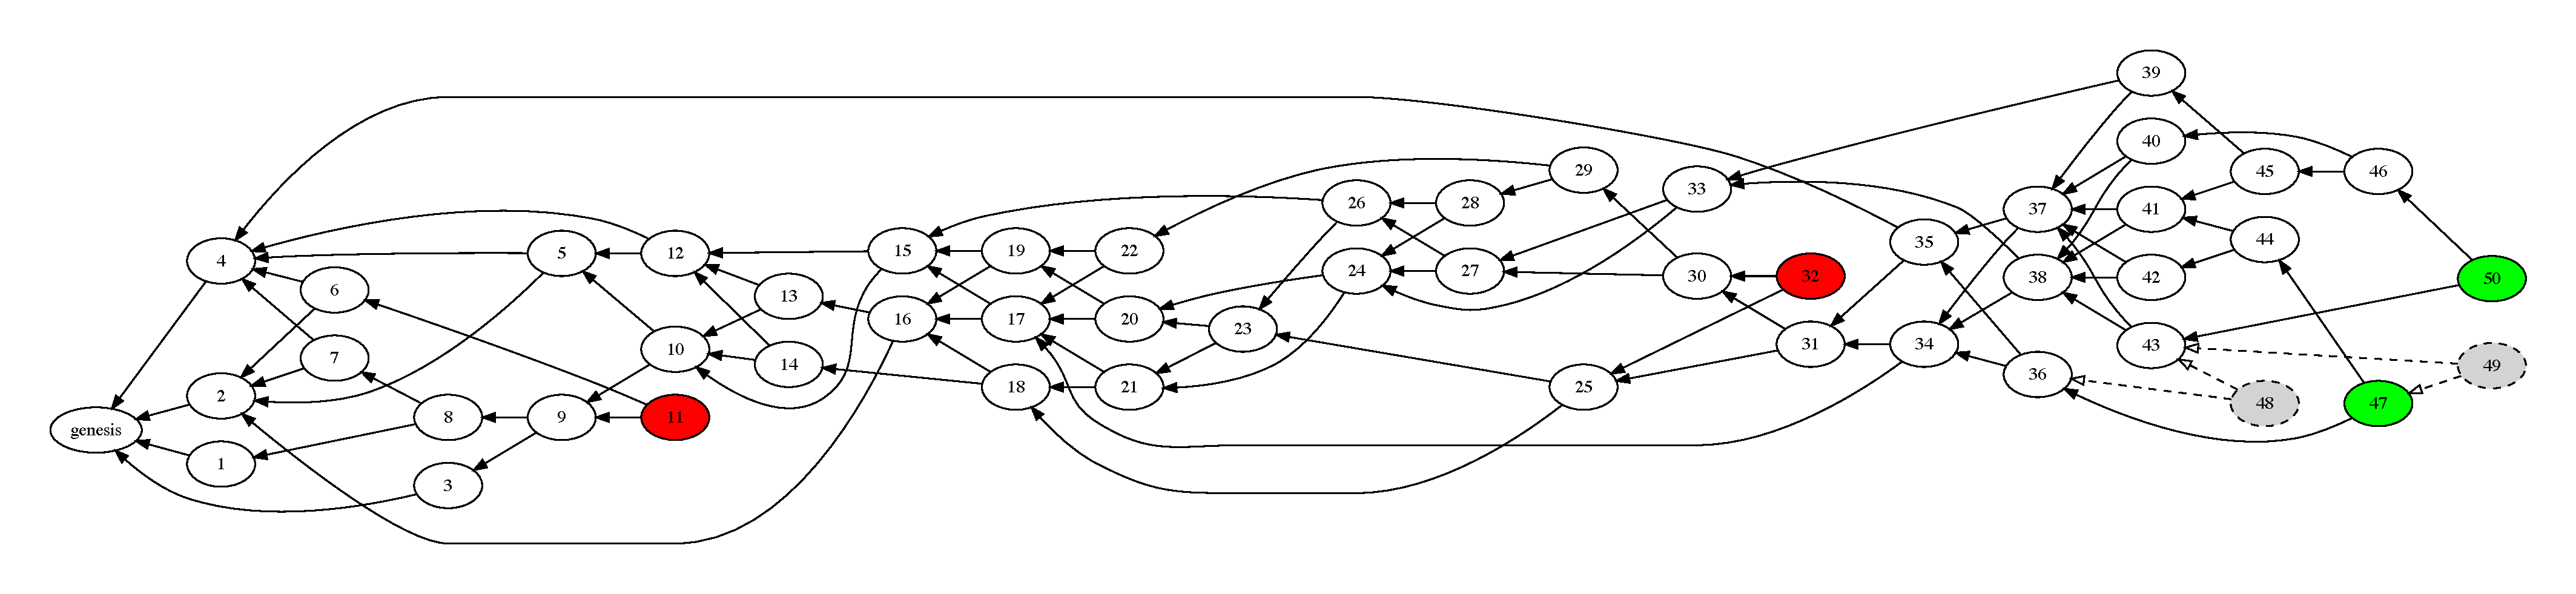
\includegraphics[width=\textwidth]{./images/fig-tangle-conflict.pdf}
\caption{The red nodes are transactions which had some conflict with previous transaction and were invalidated by the network. Notice that none of them have been confirmed.\label{fig-tangle-conflict}}
\end{figure}

\section{Nuclear submarine attack}

The nuclear submarine attack, also known as the parasite chain attack, is when the attacker generates a separate DAG (or a side DAG), with many transactions and a lot of proof-of-work. This side DAG is off the network, i.e., its transactions have not been propagated. Then, at a convenient moment, the attacker suddenly propagates these transactions. The whole network needs to decide how to handle these transactions.

If the transactions have no conflict with any transaction of the main DAG, i.e., there is no transaction spending the ``same money'', then it seems easy to handle the transactions. But, as it is an attack, probably there will be some conflicts, and it is not easy to choose which transaction should be invalidated. As the attacker has been generating a separate DAG, the conflicting transaction may have an accumulated weight similar or greater than the transaction in the main DAG. Thus, using only the accumulated weight may not be enough to prevent this attack.

For example, the attacker may generate a transaction which transfers all their funds to another address. Then, they start to generate many new transactions which confirms themselves and even confirms some of the transactions in the main DAG. But none of these transactions are propagated to the network. Then, the attacker buys something in the real world, pays with cryptocurrency, and wait until the payment gets the accumulated weight demanded by the merchant. Finally, the attacker suddenly propagates all the transactions to the network in a small window of time. This may cause the network to accept the attacker's original transaction instead of the one used to pay the merchant. Hence, the merchant transaction is invalidated, and the double spend attack has succeeded.

\section{Proposal: Questions to be explored}

Given these preliminaries, these are some questions with which we will be concerned.

In this paper, we will analyze the network scaling and security. How a DAG network scales, simulating different loads and measuring the bandwidth, computational effort, and storage space necessary to handle all the transactions in time. What is the minimum transaction's aggregated weight which it may be considered unlikely to be reversed?

We are interested in how the rate of new transactions affects how long it takes to a new transaction to be confirmed for the first time. We had already run some simulations under normal load (Fig. \ref{fig-tangle-hist}) and high load (Fig. \ref{fig-tangle-hist-2}).

\begin{figure}[ht]
\centering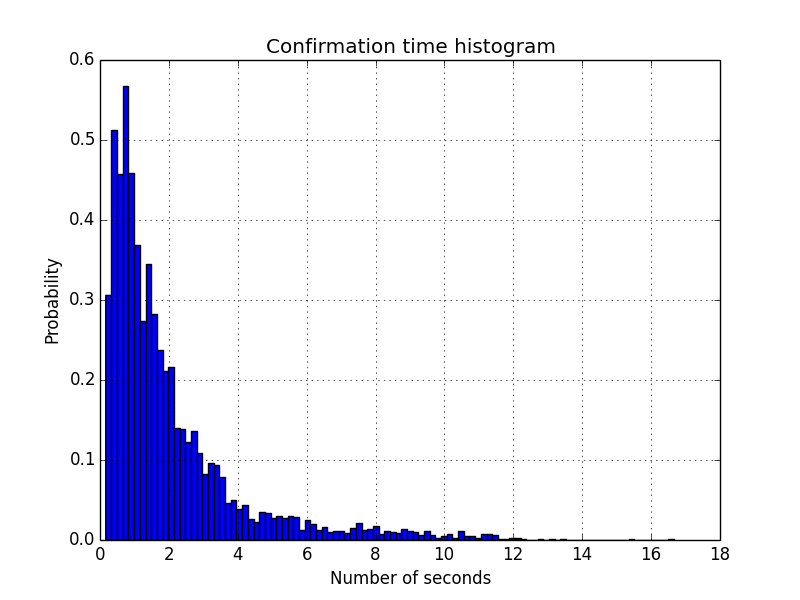
\includegraphics[width=\textwidth]{./images/fig-tangle-hist.png}
\caption{Histogram of how long has been a transaction waiting until its first confirmation. It was a simulation of 15 minutes with new transactions rate changing between 1 and 15 tx/s.\label{fig-tangle-hist}}
\end{figure}

\begin{figure}[ht]
\centering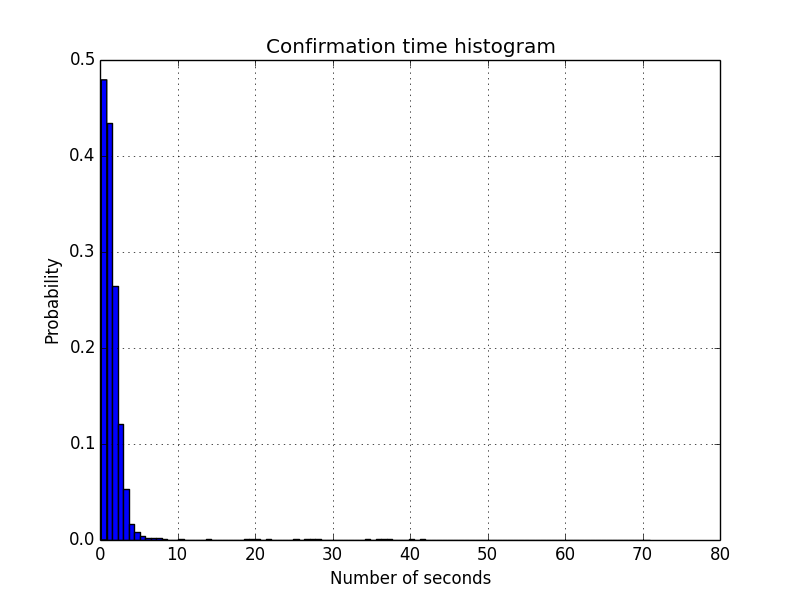
\includegraphics[width=\textwidth]{./images/fig-tangle-hist-2.png}
\caption{Histogram of how long has been a transaction waiting until its first confirmation. It was a simulation of 5 minutes with new transactions rate of 50 tx/s, i.e., very high load.\label{fig-tangle-hist-2}}
\end{figure}


Besides the time to the first confirmation, it is also important to measure how long it takes to a new transaction reach a specific accumulated weight. It is useful for exchanges and merchants to set their minimum requirements. Bitcoin's exchanges and merchants usually requires a minimum of 6 confirmations blocks.

As the DAG network is distributed, its users may use different parameters --- they cannot violate the network's rules, but they may use different tip selection algorithms, for instance. We would like to explore how different users' parameters may affect the network, how much is necessary to cause either a hard-fork or a soft-fork.

\cite{tangle2016} suggests that constraining transactions' weight in a range would both prevent spam, because it would be necessary a minimum work to propagate a new transaction, and attacks, because an attacker would not be allowed to propagate a transaction with very high weight. We agree with the spam argument, and would like how a minimum weight would affect mobile devices's new transactions. We partially agree with the upper bound, because an attacker would be able to generate many transaction with lower weight. We will analyze if constraining transactions' weight would be effective against nuclear submarine attacks.

We have another suggestion to prevent nuclear submarine attacks: set a maximum depth for the transactions confirmed by a new transaction. So, new transactions would have to confirming newer transactions instead of old transactions, and a nuclear submarine attack would be controlled because the attacker would be not be able to create a large separate DAG. But the maximum depth rule would possibly also affect transaction created by low (hash)power devices, because it would take a longer time to solve the proof-of-work and, if the confirmations are going fast, the transaction would possibly be invalidated. This raises another important question: what would be an optimal maximum depth allowed?

If we would like to include fee transactions, how would it be distributed between confirmations? As transactions may have multiple direct confirmations, it is not obvious who would receive the transaction fee. An intuitive suggestion would be to give the fee to the first confirmation with a minimum weight, but it might have some propagation problems, because it takes a while to propagate a transaction in the network and there would be conflict.

In order to solve the fee distribution problem, we will simulate how the network would behave if we include blocks. These blocks would be like Bitcoin's, with an adjustable proof-of-work according to the network's hashpower. They would receive the fees from all confirmed transactions which had not been confirmed by any block before, and they would be able to generate new coins. These blocks would also help solving other problems.

%\begin{enumerate}
%\item Which parameters turns the network more or less vulnerable to attacks?
%\item Is there an optimal strategy to attack?
%\item Could new coins be generated demanding a proof-of-work with dynamic difficulty, like in Bitcoin?
%\item What is the equation of number of tips over time? What is the equation of how long it takes to a transaction to be confirmed for the first time? What is the equation of the accumulated weight of a transaction over time? Some equations have already been proposed by \citet{tangle2016}.
%\end{enumerate}

\chapter{Methodology}

The methodology we have been using is computer simulation. Through the simulation of many scenarios of DAG model with different parameters, we will understand how the network behaves in complex scenarios, mainly when the load is suddenly increased, and when the network is under attack. We will first test our hypothesis through simulation and than prove them mathematically.

The simulator has been developed using an event-based design which is capable of running hours of simulation in just a few minutes. It creates agents who decide to make a transaction, then they select which transactions will be confirmed, then they spend some time working in the proof-of-work, and, finally, they propagate the transaction to the network. The other agents receive the transaction and may accept or deny it. The agents may use different parameters among themselves.

When a new transaction is added to the DAG, it uses a depth-first search \citep{cormen2009introduction} (i) to update the aggregated weight of the directly and indirectly confirmed transactions, (ii) to calculate its own score, and (iii) to generate a topological sort \citep{cormen2009introduction}. The topological sort is used to calculate the longest path from all other transactions to the new transaction, and this longest path is used to update the depth of the whole DAG. If the new transaction confirms only transactions which has already been confirmed, the depth update is skipped thanks to Theorem \ref{theorem-new-tx-not-tip}.

The necessary time to generate the proof-of-work is estimated by the function $k \cdot 2^{weight}$, where $k$ is a constant related to the computing power of the agent and weight is randomly chosen.

The time between two new transactions is sampled from the exponential distribution with parameter $\lambda$. The value of $\lambda$ is changed over time, causing changes in the load of the network. We consider 1 tx/s to be a low load, and 15 tx/s to be a high load. Even though we have already tested up to 100 tx/s.

The simulator will output different reports: (i) snapshots of the DAG at interesting moments, such as Fig. \ref{fig-tangle-example}, \ref{fig-tangle-swarm}, and \ref{fig-tangle-conflict}; (ii) histogram of confirmation time, such as Fig. \ref{fig-tangle-hist} and \ref{fig-tangle-hist-2}; and many others.

\section{Proposal: Theorems to be proved}

The following theorems will be mathematically proved. They have already been used in the implementation of the simulator.

\begin{theorem}
\label{theorem-new-tx-not-tip}
When a new transaction confirms an already confirmed transaction, the depth of all transactions remains the same, i.e., the depth of the transactions are only changed when a new transaction confirm an unconfirmed transaction.
\end{theorem}

\begin{theorem}
The height of a transaction is equal to the maximum height of its parents plus one.
\end{theorem}

\begin{theorem}
If new transactions choose randomly the unconfirmed transactions to be confirmed, then no unconfirmed transaction will be left behind, i.e., all transactions will be confirmed in due time.
\end{theorem}

\chapter{Conclusion}

Bitcoin's underlying technology blockchain has been called by many as a major invention comparable to the invention of the internet. But it is unlikely that Bitcoin and blockchain have achieved the final or most optimal design for a secure and scalable electronic transaction system. In this work, we will investigate whether DAG model is suitable to be a real alternative to blockchain.

Preliminary results obtained from our simulator have shown that, using a random tip selection strategy, the network seems to support up to 50 transactions per second, with no tip abandoned (Fig. \ref{fig-tangle-swarm}) or taking too long to have at least one confirmation (Fig. \ref{fig-tangle-hist-2}). Today, Bitcoin network can barely handle 8 transactions per second without increasing the unconfirmed transaction list to hundreds of thousands --- several transactions take days to be confirmed.

We have not yet tested the security of the network against double spend attacks. It will be one of the next steps and we expect to block a nuclear submarine attack including a rule for invalidate new conflicting transactions which confirm transactions with depth greater than a given threshold. We are unsure whether this rule would invalidate legitimate transactions on a high load scenario.

We also plan to improve the analysis of the confirmation time. So far, we have the histograms of how long it takes to a transaction to be confirmed for the first time (Fig. \ref{fig-tangle-hist} and \ref{fig-tangle-hist-2}). We will also generate the histograms of how long it takes to a transaction to have an accumulated weight of at least a given number. It is an important histogram because it helps merchants and users to decide how long they should wait to consider the transaction almost irreversible.

We will also work on the mathematical modeling of DAG networks, and the equations will help us to understand the limits of these networks.

